\documentclass[12pt,a4paper,oneside]{article}

%\usepackage[utf8]{inputenc}
%\usepackage[T1]{fontenc}
\usepackage{etex}
\usepackage{fixltx2e}
\usepackage{graphicx}
\usepackage{longtable}
\usepackage{float}
\usepackage{wrapfig}
\usepackage{soul}
\usepackage{textcomp}
\usepackage{marvosym}
%\usepackage{wasysym}
\usepackage{latexsym}
\usepackage{amssymb}
%\usepackage{hyperref}
\tolerance=1000
\usepackage{amsmath}
\usepackage[usenames]{color}
\usepackage{pstricks}
\usepackage{pgfplots}
\usepackage{tikz}
\usepackage[europeanresistors,americaninductors]{circuitikz}
\usepackage{colortbl}
\usepackage{yfonts}
\usetikzlibrary{shapes,arrows,matrix}
\usetikzlibrary{positioning}
\usetikzlibrary{intersections}
\usetikzlibrary{calc,patterns,decorations.pathmorphing,decorations.markings}
%\usetikzlibrary{external}
%\tikzset{external/system call={xelatex \tikzexternalcheckshellescape -halt-on-error -shell-escape -interaction=batchmode -jobname "\image" "\texsource"}}
%\tikzexternalize
\usepackage[BoldFont,SlantFont,CJKchecksingle,CJKnumber]{xeCJK}
\setCJKmonofont{Evermore Kai}
\setCJKmainfont[BoldFont=Evermore Hei]{Evermore Song}
\setCJKfamilyfont{hei}{Evermore Hei}
%\usepackage{CJKnumb}
%\xeCJKsetup{CJKglue=\hspace{0pt plus .08 \baselineskip }}
\usepackage{pst-node}
\usepackage{pst-plot}
\psset{unit=5mm}
%\pdfcompresslevel=9
\DeclareGraphicsExtensions{.jpg,.pdf,.mps,.png}

%\usepackage{CJK,CJKnumb}
\usepackage{listings}
\usepackage{tabularx}
\usepackage{longtable}
\usepackage{indentfirst}                % 首行缩进宏包
\usepackage{color}                      % 支持彩色
\usepackage{listings}                   % 源代码宏包
\usepackage[perpage,symbol]{footmisc}   % 脚注控制
\usepackage{lastpage}                   % 自动记录总页数宏包,计数器为LastPage
\usepackage{fancyhdr}                   % fancyhdr宏包 页眉和页脚的相关定义
\pagestyle{empty}
\topmargin -5mm \oddsidemargin -5mm \evensidemargin -5mm \textwidth 170mm \textheight 235mm
\headsep 1em
\pagestyle{fancyplain}                  % 要在\usepackage{pageno}之前,不然页眉有一条黑线去不掉
\renewcommand{\headrulewidth}{0pt}
%\usepackage{pageno}                     % 章首页的页眉处理, 可以改为自己想要的形式 

\allowdisplaybreaks


\begin{document}



%---------------------------------------源代码------------------------------------------------
\lstset{xleftmargin=1em,xrightmargin=1em}
\lstset{commentstyle=\textit,keywordstyle=\textbf,breaklines=true,columns=flexible,mathescape=true}
\lstdefinestyle{numbers}{numbers=left,stepnumber=1,numberstyle=\small,numbersep=1em}
\lstset{language=C++}
  \lstset{%
numbers=left,stepnumber=1,numberstyle=\tiny,
  %basicstyle=\footnotesize\ttfamily,
  basicstyle=\ttfamily,
  commentstyle=\textit,
  keywordstyle=\textbf,
  identifierstyle=\slshape,
  stringstyle=\small,
  %stringstyle=\color{orange},
  breaklines=true,
%    escapechar=\#,
    emphstyle=\bfseries\color{red}
}
\renewcommand{\lstlistingname}{程序}

%\CJKcaption{GB}

\newcounter{question}
\usecounter{question}
\setcounter{question}{1}
\newcommand{\question}{{\flushleft\CJKnumber{\arabic{question}}、}\stepcounter{question}}

\begin{center}
\textbf{ \fontsize{18pt}{\baselineskip}\selectfont{西北工业大学考试试题(卷)评分标准}}\\
2016 -2017 学年第 1 学期
\end{center}

%\renewcommand{\baselinestretch}{1.0}  %会使 Tikz  画的结构图出现间断

{
\flushleft

\begin{tabular}{lll}
开课学院 \underline {\hspace{2em} 航天学院\hspace{2em} }& 课程\underline {\hspace{2em} 自动控制理论II\hspace{2em} }& 学时\underline {\hspace{2em} 32\hspace{2em} }\\
考试日期\underline {\hspace{8eM} }& 考试时间\underline {\hspace{2em} \hspace{2em} }小时 & 考试形式
$\left(\begin{array}{c}
%\mbox{开}\\
\mbox{闭}
\end{array} \right)$
$\left(\begin{array}{*{10}c}
% \mbox{A} \\
 \mbox{B} 
\end{array} \right)$卷 
\end{tabular}
}


\newcommand{\onlytest}[1]{}
\newcommand{\onlyanswer}{ }

%-----------------内容放在这里--------------------------

\question(20分){已知控制系统结构图如下所示,已知 $G(s)=\frac{s}{(s+3)^3}$, 非线性环节描述函数 $N(A)=\frac{1}{A},(A>1)$,求使系统稳定无自振的$k$取值范围。
	
	
	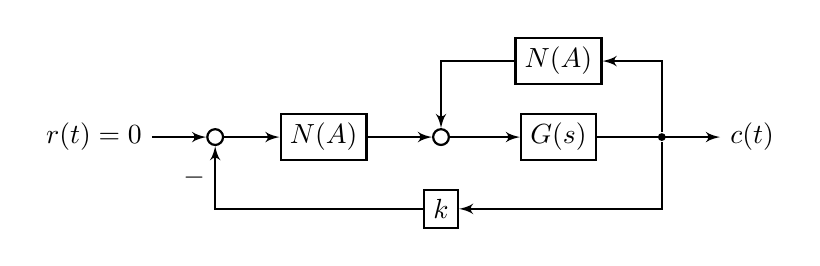
\begin{tikzpicture}[node distance=3em,auto,>=latex', thick]
	%\path[use as bounding box] (-1,0) rectangle (10,-2); 
	\tikzstyle{block} = [draw,rectangle,thick,minimum height=1em,minimum width=1em]
	\tikzstyle{sum} = [draw,circle,inner sep=0mm,minimum size=2mm]
	\tikzstyle{branch} = [circle,fill,inner sep=0pt,minimum size=1mm]
	\tikzstyle{connector} = [->,thick]
	
	\def\r{\node(r){$r(t)=0$};}
	\def\n{\node(n){$n(t)$};}
	\def\b(#1){\node[branch](b#1){};}
	\def\p(#1){\node[sum](p#1){};}
	\def\gc{\node[block](gc){$N(A)$};}
	\def\gr{\node[block](gr){$N(A)$};}
	\def\gn{\node[block](gn){$G_n(s)$};}
	\def\gp{\node[block](gp){$G(s)$};}
	\def\g(#1){\node[block](g#1){$k$};}
	\def\c{\node(c){$c(t)$};}
	
	\matrix[ampersand replacement=\&, row sep=1em, column sep=2em]{
		\&          \&     \&  \& \gr    \&   \&         \\
		\r  \&    \p(e) \& \gc \&  \p(r) \& \gp \& \b(c)  \& \c  \\
		\&         \&         \& \g(h)    \\
	};
	\draw [connector](r) -- (pe) ; 
	\draw [connector](gr) -| (pr) ;
	\draw [connector](pe) -- (gc) ; 
	\draw [connector](gc) -- (pr) ; 
	\draw [connector](pr) -- (gp) ; 
	\draw [connector](gp) -- (c) ; 
	\draw [connector](bc) |- (gr) ; 
	\draw [connector](bc) |- (gh) ; 
	\draw [connector](gh) -| node[near end , left]{$-$} (pe) ; 
	\end{tikzpicture} 
	
	\onlyanswer{
		答:
		原结构图等效为:
			
			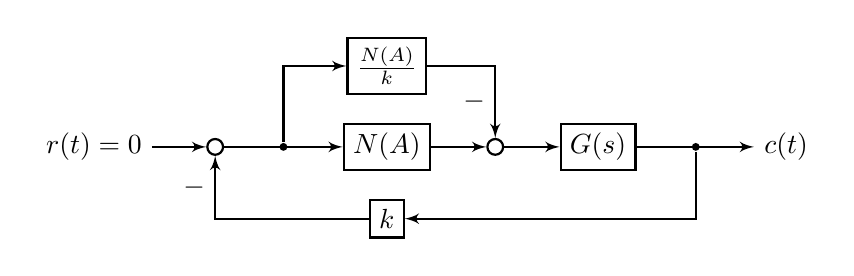
\begin{tikzpicture}[node distance=3em,auto,>=latex', thick]
			%\path[use as bounding box] (-1,0) rectangle (10,-2); 
			\tikzstyle{block} = [draw,rectangle,thick,minimum height=1em,minimum width=1em]
			\tikzstyle{sum} = [draw,circle,inner sep=0mm,minimum size=2mm]
			\tikzstyle{branch} = [circle,fill,inner sep=0pt,minimum size=1mm]
			\tikzstyle{connector} = [->,thick]
			
			\def\r{\node(r){$r(t)=0$};}
			\def\n{\node(n){$n(t)$};}
			\def\b(#1){\node[branch](b#1){};}
			\def\p(#1){\node[sum](p#1){};}
			\def\gc{\node[block](gc){$N(A)$};}
			\def\gr{\node[block](gr){$\frac{N(A)}{k}$};}
			\def\gn{\node[block](gn){$G_n(s)$};}
			\def\gp{\node[block](gp){$G(s)$};}
			\def\g(#1){\node[block](g#1){$k$};}
			\def\c{\node(c){$c(t)$};}
			
			\matrix[ampersand replacement=\&, row sep=1em, column sep=2em]{
				\&           \&  \& \gr    \&   \&         \\
				\r  \& \p(e)\& \b(r)    \& \gc \&  \p(r) \& \gp \& \b(c)  \& \c  \\
				\&         \&         \& \g(h)    \\
			};
			\draw [connector](r) -- (pe) ; 
			\draw [connector](br) |- (gr) ;
			\draw [connector](gr) -| node[near end , left]{$-$} (pr) ;
			\draw [connector](pe) -- (gc) ; 
			\draw [connector](gc) -- (pr) ; 
			\draw [connector](pr) -- (gp) ; 
			\draw [connector](gp) -- (c) ;  
			\draw [connector](bc) |- (gh) ; 
			\draw [connector](gh) -| node[near end , left]{$-$} (pe) ; 
			\end{tikzpicture} 
			
		
		两个非线性环节并联,其等效描述函数为两个环节描述函数之和。
		\begin{align*}
		N'(A) &= k(N(A)-\frac{N(A)}{k}) \\
		&= \frac{k}{A}-\frac{1}{A}\\
		-\frac{1}{N'(A)}&=-\frac{A}{k-1}\\
		\angle G(j\omega) &=90^\circ-3\angle(s+3)\\
		G(j\omega)|_{\omega=+\infty}&=0\\
		G(j\omega)|_{\omega=\sqrt{3}}&=\frac{1}{24}
		\end{align*}
		
			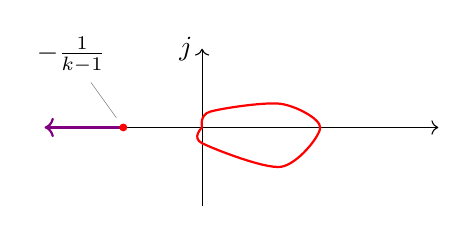
\begin{tikzpicture}[scale=1]
			\coordinate (o) at (0,0);
			\coordinate (ox) at (3,0);
			\draw[->] (-2,0) -- (ox);
			\draw[->] (0,-1) -- (0,1);
			\draw[->,violet,thick] (-1,0) -- (-2,0); % -1/N(A)=-A/(k-1)
			\draw (-1,0) node[pin=100:$-\frac{1}{k-1}$] {};
			\draw (-1,0) node [red,thick,circle,fill,inner sep=0pt,minimum size=1mm] {};
%			\draw[->,violet,thick] (2,0) -- (3,0); % -1/N(A)=-A/(k-1)
%			\draw (2,0) node[pin=100:$-\frac{1}{k-1}$] {};
%			\draw (2,0) node [red,thick,circle,fill,inner sep=0pt,minimum size=1mm] {};
			\draw [red,thick,smooth] plot coordinates {(0,0)(0.1,0.2)(1,0.3)(1.5,0)(1,-0.5)(0,-0.2) (0,0) }; %G(s)=s/(3+s)^3
%			\draw[->,red,dashed,thick] (2,0) arc (0:-100:2.5);
			\draw (0,1) node[left] {$j$};
			\end{tikzpicture}
					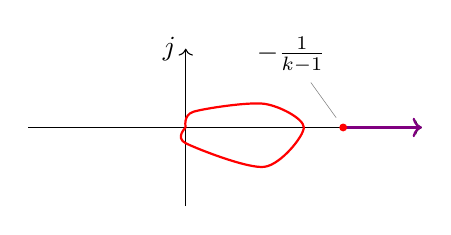
\begin{tikzpicture}[scale=1]
					\coordinate (o) at (0,0);
					\coordinate (ox) at (3,0);
					\draw[->] (-2,0) -- (ox);
					\draw[->] (0,-1) -- (0,1);
%					\draw[->,violet,thick] (-1,0) -- (-2,0); % -1/N(A)=-A/(k-1)
%					\draw (-1,0) node[pin=100:$-\frac{1}{k-1}$] {};
%					\draw (-1,0) node [red,thick,circle,fill,inner sep=0pt,minimum size=1mm] {};
					\draw[->,violet,thick] (2,0) -- (3,0); % -1/N(A)=-A/(k-1)
					\draw (2,0) node[pin=100:$-\frac{1}{k-1}$] {};
					\draw (2,0) node [red,thick,circle,fill,inner sep=0pt,minimum size=1mm] {};
					\draw [red,thick,smooth] plot coordinates {(0,0)(0.1,0.2)(1,0.3)(1.5,0)(1,-0.5)(0,-0.2) (0,0) }; %G(s)=s/(3+s)^3
					%			\draw[->,red,dashed,thick] (2,0) arc (0:-100:2.5);
					\draw (0,1) node[left] {$j$};
					\end{tikzpicture}
						
		当 $-\frac{1}{N'(A)}<0$ 或 $-\frac{1}{N'(A)}>\frac{1}{24}$ 时,系统稳定无自振,得:
		\begin{align*}
		-\frac{A}{k-1} &< 0 \\
		k&>1 
		\end{align*}
		或
		\begin{align*}
		-\frac{A}{k-1} &>\frac{1}{24} \\
		\end{align*}
		得:
			$$ -23<k<1$$ 
		系统稳定无自振时 
		$$k>-23$$
		
		
	}
}


\question(20分){单位负反馈控制系统开环传递函数:
	$$G(s)=\frac{0.01s+1}{(0.5s+1)(s+1)(10s+1)}$$
	串联校正网络:
	$$G_c(s)=k_P +\frac{k_I}{s}+k_D s$$
	若要求校正后系统开环传递函数满足:
	$$G'(s)\approx\frac{2}{s(0.5s+1)}$$
	求解参数 $k_P,k_I,k_D$。
	
	\onlyanswer
	{
		答:
		\begin{align*}
		G'(s)&\approx G(s)G_c(s)\\
		G_c(s)&\approx \frac{G'(s)}{G(s)}\\
		&\approx \frac{2(10s+1)(s+1)}{s(0.01s+1)}
		\end{align*}
		截止频率 $\omega_c \approx 2$ , 得
		\begin{align*}
		G_c(s)&\approx \frac{2(10s+1)(s+1)}{s}\\
		&\approx 2\cdot \frac{10s^2+11s+1}{s}\\
		&\approx 22+20s+\frac{2}{s}
		\end{align*}
		得:
		\begin{align*}
		k_P&=22\\
		k_D&=20\\
		k_I&=2
		\end{align*}
	}
}


\question(20分){已知控制系统结构图如下所示,已知 $G(s)=\frac{1}{s-11}, G_c(s)=k, G_r(s)=\frac{a s+b}{s+1}$ 。如何选取$k,G_n(s)$能够完全消除扰动 $n(t)$ 对系统的影响?当$r(t)=sin(t),n(t)=0,(t>0)$时, 是否存在 $k,a,b$ 使稳态误差为零?

	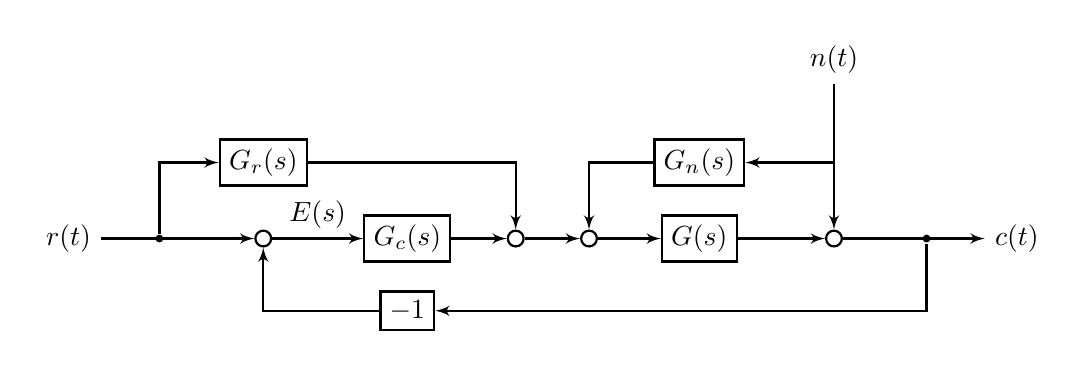
\begin{tikzpicture}[node distance=3em,auto,>=latex', thick]
	%\path[use as bounding box] (-1,0) rectangle (10,-2); 
	\tikzstyle{block} = [draw,rectangle,thick,minimum height=1em,minimum width=1em]
	\tikzstyle{sum} = [draw,circle,inner sep=0mm,minimum size=2mm]
	\tikzstyle{branch} = [circle,fill,inner sep=0pt,minimum size=1mm]
	\tikzstyle{connector} = [->,thick]
	
	\def\r{\node(r){$r(t)$};}
	\def\n{\node(n){$n(t)$};}
	\def\b(#1){\node[branch](b#1){};}
	\def\p(#1){\node[sum](p#1){};}
	\def\gc{\node[block](gc){$G_c(s)$};}
	\def\gr{\node[block](gr){$G_r(s)$};}
	\def\gn{\node[block](gn){$G_n(s)$};}
	\def\gp{\node[block](gp){$G(s)$};}
	\def\g(#1){\node[block](g#1){$-1$};}
	\def\c{\node(c){$c(t)$};}
	
	\matrix[ampersand replacement=\&, row sep=1em, column sep=2em]{
		\&          \&        \&     \&       \&        \&    \& \n \\
		\\
		\&          \&   \gr  \&     \&       \&        \& \gn \\
		\r  \&   \b(r)  \& \p(e)  \& \gc \& \p(r) \&  \p(n) \& \gp \& \p(c) \& \b(c)  \& \c  \\
		\&         \&         \& \g(h)    \\
	};
	\draw [connector](r) -- (pe) ; 
	\draw [connector](n) -- (pc) ; 
	\draw [connector](n) |- (gn) ; 
	\draw [connector](br) |- (gr) ; 
	\draw [connector](gr) -| (pr) ;
	\draw [connector](gn) -| (pn) ; 
	\draw [connector](pe) -- node[midway]{$E(s)$} (gc) ; 
	\draw [connector](gc) -- (pr) ; 
	\draw [connector](pr) -- (pn) ; 
	\draw [connector](pn) -- (gp) ; 
	\draw [connector](gp) -- (pc) ; 
	\draw [connector](pc) -- (c) ; 
	\draw [connector](bc) |- (gh) ; 
	\draw [connector](gh) -| node[near end , left]{$ $} (pe) ; 
	\end{tikzpicture} 
	
	\onlyanswer
	{
		答:
		
		\begin{align*}
		\frac{E(s)}{N(s)}&=-\frac{1+G_n(s)G(s)}{1+G_c(s)G(s)}\\
		&=-\frac{1+\frac{G(s)}{s-1}}{1+\frac{k}{s-1}}
		&=-\frac{s-1+G(s)}{s-1+k}
		\end{align*}
		$\frac{E(s)}{N(s)} =0$时,扰动对系统无影响,得:$G(s)=1-s$。


        当$r(t)=sin(t),n(t)=0,(t>0)$时,
		\begin{align*}
		E(s)&=\frac{1-G_r(s)G(s)}{1+G_c(s)G(s)}\cdot R(s)\\
		&=\frac{1-\frac{as+b}{s+1}\frac{k}{s-1}}{1+\frac{k}{s-1}}\cdot\frac{1}{s^2+1}\\
		&=\frac{s-1-\frac{k(as+b)}{s+1}}{s-1+k}\cdot\frac{1}{s^2+1}\\
		&=\frac{s^2-1-k(as+b)}{(s-1+k)(s+1)}\cdot\frac{1}{s^2+1}
		\end{align*}
		选取 $k>1,a=0,b=\frac{-2}{k}$ ,得:
		\begin{align*}
		E(s)&=\frac{s^2+1}{(s-1+k)(s+1)}\cdot\frac{1}{s^2+1}\\
		&=\frac{1}{(s-1+k)(s+1)}\\
		\lim_{s\to 0}sE(s)&=0
		\end{align*}
		稳态误差为零。
	}
}

\question(20分){已知控制系统结构图如下所示,求 $C(z),\hat{C}(z)$

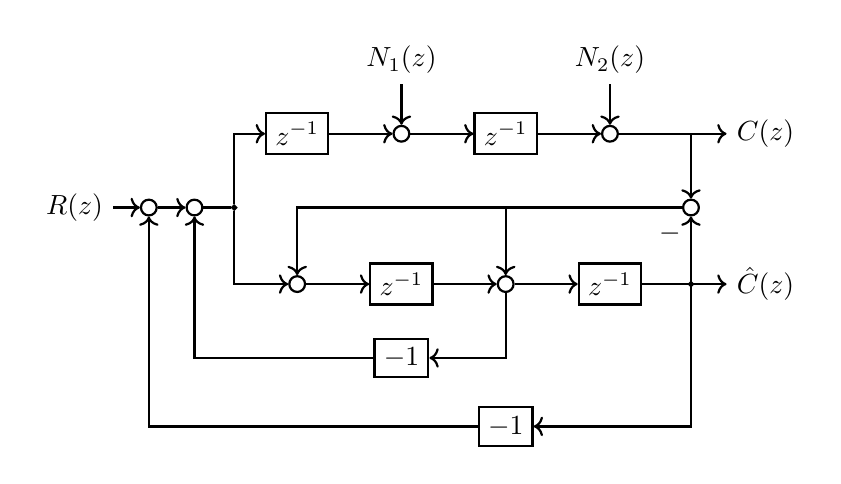
\begin{tikzpicture}[scale=1, thick] 
\tikzstyle{block} = [draw,rectangle,thick,minimum height=1em,minimum width=1em]
\tikzstyle{sum} = [draw,circle,inner sep=0mm,minimum size=2mm]
\tikzstyle{branch} = [draw,fill,circle,inner sep=0pt,minimum size=0.5mm]
\tikzstyle{connector} = [->,thick]
\matrix[ampersand replacement=\&, row sep=1em, column sep=1em]{
	\&\&\&\&\& \node(n1){$N_1(z)$};\&\&\node(n2){$N_2(z)$}; \\
	
	\&\&\&\& \node[block](g1){$z^{-1}$}; \& \node[sum](pn1) {}; \& \node[block] (g2){$z^{-1}$}; \& \node[sum](pn2) {};  \&
	\& \node[] (c){$C(z)$};\\
	
	\node[] (r) {$R(z)$}; \& 
	\node[sum](pe1) {};\&
	\node[sum](pe2) {};\&
	\node[branch] (b1) {} ; \&\&\&\&\&
	\node[sum](pe3) {};\\
	
	\&\&\&\& \node[sum](ps1) {}; \& 
	\node[block](g3){$z^{-1}$}; \& 
	\node[sum](ps2) {}; \& \node[block](g4){$z^{-1}$};\&
	\node[branch] (b2) {} ;  \& \node[] (hatc){$\hat{C}(z)$}; \\
	
	\&\&\&\&\& \node[block](h1) {$-1$}; \\
	\&\&\&\&\&\& \node[block](h2){$-1$}; \\
};
\draw [connector] (n1) -- (pn1);
\draw [connector] (n2) -- (pn2);
\draw [connector] (r) -- (pe1);
\draw [connector] (pe1) -- (pe2);
\draw [thick] (pe2) -- (b1);
\draw [connector] (b1) |- (g1);
\draw [connector] (b1) |- (ps1);
\draw [connector] (ps1) -- (g3);
\draw [connector] (g1) -- (pn1);
\draw [connector] (pn1) -- (g2);
\draw [connector] (g3) -- (ps2);
\draw [connector] (ps2) -- (g4);
\draw [connector] (g2) -- (pn2);
\draw [connector] (pn2) -| (pe3);
\draw [connector] (pn2) -- (c);
\draw [connector] (g4) -|   node[very near end,left] {$-$} (pe3);
\draw [connector] (g4) -- (hatc);
\draw [connector] (pe3) -| (ps1);
\draw [connector] (pe3) -| (ps2);
\draw [connector] (ps2) |- (h1);
\draw [connector] (b2) |- (h2);
\draw [connector] (h1) -|  node[very near end,left] {$ $} (pe2);
\draw [connector] (h2) -|  node[very near end,left] {$ $} (pe1);
\end{tikzpicture} 

\onlyanswer
{
	答:设 $E(z)=C(z)-\hat{C}(z)$,得:
	\begin{align*}
	z\hat{C}(z) &= \frac{R(z)-\hat{C}(z)-z\hat{C}(z)+E(z)}{z}+E(z) \\
	z\hat{C}(z)+\hat{C}(z)+\frac{\hat{C}(z)}{z}&= \frac{R(s)+zE(z)+E(z)}{z}\\
	(z^2+z+1)\hat{C}(z) &=R(z)+(z+1)E(z)\\
	\hat{C}(z) &=\frac{R(z)+(z+1)E(z)}{z^2+z+1}
	\end{align*}
	及:
	\begin{align*}
	C(z) &= \frac{R(z)-\hat{C}(z)-z\hat{C}(z)}{z^2}+\frac{N_1(z)}{z}+N_2(z)\\
	z^2 C(z) &= R(z)-(z+1)\hat{C}(z)+zN_1(z)+z^2 N_2(z)\\
	z^2 C(z) &= R(z)-(z+1)(C(z)-E(z))+zN_1(z)+z^2 N_2(z)\\
	(z^2+z+1) C(z) &= R(z)+(z+1)E(z)+zN_1(z)+z^2 N_2(z)\\
	C(z) &= \frac{R(z)+(z+1)E(z)+zN_1(z)+z^2 N_2(z)}{z^2+z+1}
	\end{align*}
	
	得:
	\begin{align*}
	\hat{C}(z) &=\frac{R(z)+(z+1)E(z)}{z^2+z+1}\\
	C(z) &= \frac{R(z)+(z+1)E(z)+zN_1(z)+z^2 N_2(z)}{z^2+z+1}\\
	E(z) &=\frac{zN_1(z)+z^2 N_2(z)}{z^2+z+1}\\
	\hat{C}(z) &=\frac{R(z)}{z^2+z+1}+\frac{(z+1)(zN_1(z)+z^2 N_2(z))}{(z^2+z+1)^2}\\
	C(z) &= \frac{R(z)+zN_1(z)+z^2 N_2(z)}{z^2+z+1}+\frac{(z+1)(zN_1(z)+z^2 N_2(z))}{(z^2+z+1)^2}
	\end{align*}
	
}
}

%\onlytest{\vskip 3em}

%\onlytest{\newpage}


\question(20分) { 已知控制系统结构图如下所示, 分析使系统稳定的 $k_1,k_2$ 取值范围;当$r(t)=\delta(t)$时,给出$E(z)$的表达式。

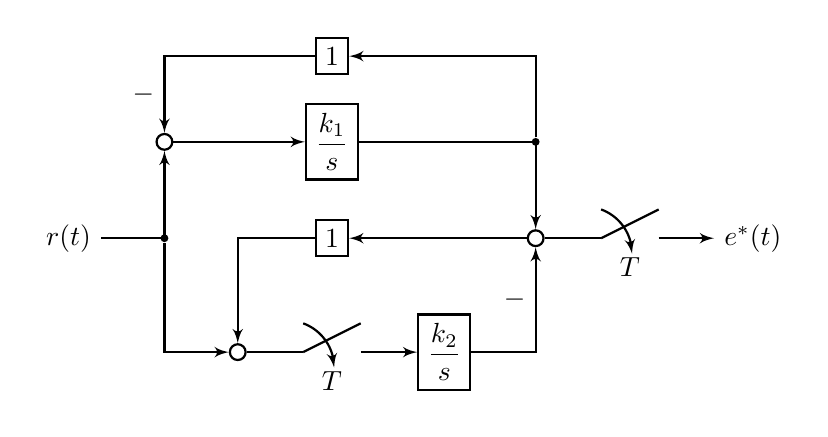
\begin{tikzpicture}[node distance=3em,auto,>=latex', thick]
%\path[use as bounding box] (-1,0) rectangle (10,-2); 
\tikzstyle{block} = [draw,rectangle,thick,minimum height=1em,minimum width=1em]
\tikzstyle{sum} = [draw,circle,inner sep=0mm,minimum size=2mm]
\tikzstyle{branch} = [circle,fill,inner sep=0pt,minimum size=1mm]
\tikzstyle{connector} = [->,thick]

\def\r{\node(r){$r(t)$};}
\def\rd{\node(rd){$r^*(t)$};}
\def\b(#1){\node[branch](b#1){};}
\def\p(#1){\node[sum](p#1){};}
\def\s(#1){\path[->] node[minimum size=2em] (s#1) {}; \draw (s#1.west)--(s#1.north east);\draw[->] (s#1.north west) arc (70:0:1.7em);\draw (s#1.south) node {$T$};}
\def\sd(#1){\path[->] node[minimum size=2em] (sd#1) {}; \draw[dashed] (sd#1.west)--(sd#1.north east);\draw[dashed,->] (sd#1.north west) arc (70:0:1.7em);\draw[dashed] (sd#1.south) node {$T$};}
\def\gc{\node[block](gc){$\dfrac{k_1}{s}$};}
\def\gd{\node[block](gd){$\dfrac{k_2}{s}$};}
\def\gh0{\node[block](gh0){$\dfrac{1-e^{-sT}}{s}$};}
\def\g(#1){\node[block](g#1){$1$};}
\def\ed{\node(ed){$e^*(t)$};}

\matrix[ampersand replacement=\&, row sep=1em, column sep=2em]{
	\&    \&        \& \g(ch)    \\
	\&    \p(ce) \&  \& \gc  \&  \& \b(c)  \\
	\r  \&   \b(r)  \&   \& \g(h)  \&   \& \p(e) \& \s(e)  \&  \ed  \\
	\&   \&   \p(r) \& \s(de)   \& \gd  \&    \\  
	%\&         \&   \& \g(dh)    \\
};
\draw [connector](r) -| (pce) ; 
\draw [connector](br) |- (pr) ; 
\draw [connector](pce) -- (gc) ; 
\draw [connector](gc) -| (pe) ; 
\draw [connector](bc) |- (gch) ; 
\draw [connector](gch) -| node[near end , left]{$-$} (pce) ; 
%\draw [connector](pde) -- (pr) ;  
\draw [](pr) -- (sde) ;  
\draw [connector](sde) -- (gd) ;  
\draw [connector](gd) -| node[near end , left ]{$-$} (pe) ; 
%\draw [connector](bd) |- (gdh) ; 
%\draw [connector](gdh) -| node[near end , left ]{$-$} (pde) ; 
\draw [](pe) -- (se) ; 
\draw [connector](se) -- (ed) ; 
\draw [connector](pe) -- (gh) ; 
\draw [connector](gh) -| (pr) ; 
\end{tikzpicture} 


常见 $Z$ 变换表:
$$
\begin{array}{ccc}
f(t)     &   F(s)  &  F(Z)   \\ 
\delta(t)   &   1      &  1    \\  
1(t)         &   \frac{1}{s} &  \frac{1}{1-z^{-1}}   \\ 
t            &   \frac{1}{s^2} &  \frac{Tz^{-1}}{(1-z^{-1})^2}   \\  
e^{-at}      &   \frac{1}{s+a} &  \frac{1}{1-e^{-aT}z^{-1}}  \\ 
a^{t/T}      &   \frac{1}{s-(1/T)\ln a} & \frac{1}{1-az^{-1}} 
\end{array}
$$

\onlyanswer
{
	答:由结构图可知:
	\begin{align*}
	E^*(s) &= \left[R(s)\frac{k_1}{s+k_1}-(R^*(s)+E^*(s))\frac{k_2}{s}\right]^* \\
	&=\left[\frac{R(s)k_1}{s+k_1}\right]^*-R^*(s)\left[\frac{k_2}{s}\right]^*-E^*(s)\left[\frac{k_2}{s}\right]^*
	\end{align*}
	当$r(t)=\delta(t)$时
	\begin{align*}
	E^*(s)&=\left[\frac{k_1}{s+k_1}\right]^*-\left[\frac{k_2}{s}\right]^*-E^*(s)\left[\frac{k_2}{s}\right]^*\\
	E(z)&=\frac{k_1}{1-e^{-k_1T}z^{-1}}-\frac{k_2}{1-z^{-1}}-E(z)\frac{k_2}{1-z^{-1}}\\
	&=\frac{\frac{k_1}{1-e^{-k_1T}z^{-1}}-\frac{k_2}{1-z^{-1}}}{1+\frac{k_2}{1-z^{-1}}}\\
	&=\frac{k_1(1-z^{-1})-k_2(1-e^{-k_1T}z^{-1})}{(1-z^{-1}+k_2)(1-e^{-k_1T}z^{-1})}\\
	\end{align*}
	特征根:
	\begin{align*}
	\lambda_1 &=\frac{1}{k_2+1}\\
	\lambda_2 &=e^{-k_1T}
	\end{align*}
	当 $k_1\in(0,+\infty),k_2\in(1,+\infty)\cup(-\infty,-2)$ 时系统稳定。
}

}


%-------------------------------------------------------
\clearpage


\end{document}
